\subsection{Keys and Addresses}\label{section: zk-zkvm-keys-addresses}

Encryption schemes and signature schemes in cryptography are the basis for achieving privacy. Encryption schemes include symmetric encryption and asymmetric encryption. In symmetric encryption, the sender and recipient first agree with a secret between them using key agreement scheme, and then derive a symmetric key from the secret for encryption and decryption. In asymmetric encryption, the sender encrypts the plaintext with the recipient's public key, and then the recipient decrypts the ciphertext with his own private key. The signature scheme is just the opposite, the sender signs plaintext with his own private key, and others can use the sender's public key to verify the signature.

A variety of encryption and signature schemes are used in Ola to protect privacy. At the same time, in order to enable the separation of spending and viewing permissions, some new keys are derived based on the elliptic curve algorithm, which constitutes Ola's key system.

\begin{figure}[!htp]
    \centering
    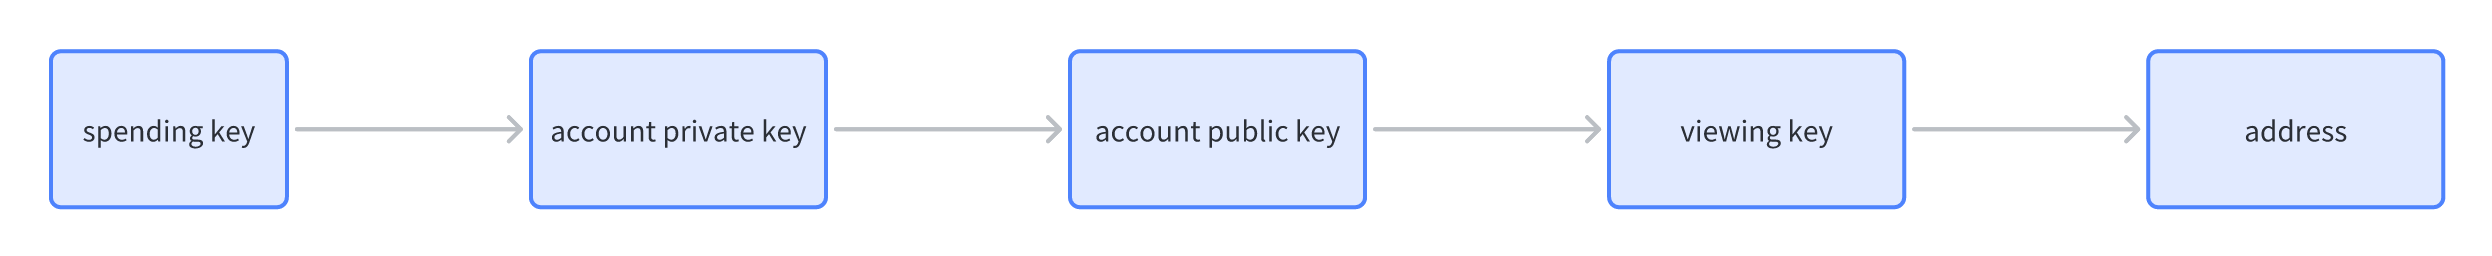
\includegraphics[width=0.8\textwidth]{key_system.png}
    \caption{Key system of Ola}
    \label{fig: key_system}
\end{figure}

\subsubsection{Spending Keys}\label{section: spending-keys}

Spending keys are the most important keys in the key system. Similar to the private keys in Bitcoin, whoever owns the spending key can spend and view the balance and transaction history in the address associated with this key. The Spending key is used to generate other keys, which is essentially a 256-bit random number, which makes it as secure as Bitcoin in some respects.
\subsubsection{Account Private Keys}\label{section: account-private-keys}

Account private keys are derived from the associated spending keys. Account private keys are private keys just like the spending keys and can not be leaked to others. A Account private key can be used to sign transactions and generate note commitments. It mainly consists of three parts:

\begin{itemize}
    \item Random commitment key
        \begin{itemize}
            \item a random number used in commitment scheme
        \end{itemize}
    \item Signature secret key
        \begin{itemize}
            \item A key used in signature scheme
        \end{itemize}
    \item Random seed
        \begin{itemize}
            \item A random number seed
            \item Signature secret key and rcm are all derived from a rseed
        \end{itemize}
\end{itemize}

The random commitment key is a scalar used in commitment schemes. The signature secret key is also a scalar used for private keys in signature schemes. The random seed is a random number generated by a random number generator, which is an element in a finite field and is 32 bytes in size.
\subsubsection{Account Public Keys}\label{section: account-public-keys}

Account public keys are derived from the associated account private keys, which mainly includes:

\begin{itemize}
    \item Signature public key
    \item Signature public random key
    \item PRF secret key
\end{itemize}

The signature public key is a public key derived from the generator G of the group on an elliptic curve and a signature secret key, which is essentially a group element on the elliptic curve, and is used to verify the signature in a signature scheme
\[ \mathrm{Sig\_Pub\_Key} = G^{\mathrm{Sig\_Pri\_Key}} \]

The signature public random key is a random number derived from random commitment key for a signature scheme, and is essentially an element of the group defined on the elliptic curve
\[ \mathrm{Sig\_Pub\_Rand} = G^{\mathrm{rcm}} \]

The PRF secret key is a key used in the Pseudo Random Function to generate pseudo-random numbers
\[ \mathrm{PRF}_{sk}(x) = \mathrm{Hash}(sk \mathbin{||} x) \]

\subsubsection{Viewing Keys}\label{section: viewing-keys}

Viewing keys are derived from associated account private keys, and each viewing key can generate one or more addresses. A viewing key can decrypt all transaction records associated with its address, that is, arbitrarily read transaction data under the address, so they can be used by regulatory departments to audit the historical transactions of an account. It can also be handed over to an delegate to generate zero-knowledge proofs. After the viewing key is leaked, all transaction data will be traced, but no assets will be lost (only the account private key can spend the user's assets). Viewing keys can only be issued to trusted institutions.

The viewing key is derived directly from the user's account private key
$$viewing\_key = private\_key.sk + private\_key.rcm + public\_key.sk\_prf$$

The main reason for creating a viewing key is to separate spending permissions and viewing permissions for user addresses. Users can share the viewing key with others to help themselves when necessary (such as asking delegates to generate zero-knowledge proofs for themselves), while keeping the spend key private.
\subsubsection{Addresses}\label{section: addresses}

Addresses are generated by associated account public keys or viewing keys to receive transfers. Addresses in Ola are either transparent or shielded (private). Transparent addresses are publicly visible on the blockchain, in the same way that Bitcoin addresses are viewable. Shielded addresses are invisible and transactions between shielded addresses do not reveal either address, the transaction value or the content of the encrypted field.

Zcash has defined a mechanism for generating hierarchical deterministic wallets in \href{https://zips.z.cash/zip-0032}{ZIP 32}, just like \href{https://github.com/bitcoin/bips/blob/master/bip-0032.mediawiki}{BIP 32}. It can help users who want to generate multiple addresses per account. All derivations produce an opaque binary spending key, from which the keys and addresses are then derived.

\begin{itemize}
    \item ZIP 32
        \begin{itemize}
            \item Account 0
                \begin{itemize}
                    \item Diversified address 0
                    \item Diversified address 1
                    \item ...
                \end{itemize}
            \item Account 1
                \begin{itemize}
                    \item Diversified address 0
                    \item Diversified address 1
                    \item ...
                \end{itemize}
            \item ...
        \end{itemize}
\end{itemize}

Ola will also design a similar mechanism in the future to implement a lightweight diversified address derivation scheme, which provides different payment addresses to different senders when users receive money to better protect the privacy of users.